\documentclass[11pt]{article}
\usepackage{hyperref}
\usepackage{amsmath}
\usepackage{bm}
\usepackage{cleveref}
\usepackage[totalwidth=450pt, totalheight=630pt]{geometry}
\usepackage[round]{natbib}
\usepackage{parskip}
\usepackage{graphicx}
\graphicspath{{figures/}}
\newcommand{\expnum}[2]{{#1}\mathrm{e}{#2}}

% Remove when finished
\usepackage{color}
\newcommand{\todo}[1]{\textcolor{red}{(TODO: #1)}}

\title{Referee Report on \citet{Pitt:2016cu}: Statistical Analysis of Numerical Preclinical Radiobiological Data} 

\author{Madeleine Sheehan \\ {\tt m.sheehan@berkeley.edu}
\and Kenneth Hung \\ {\tt kenhung@berkeley.edu}
\and Yiyi Chen \\ {\tt yiyi.chen@berkeley.edu}
\and Yulin Liu \\ {\tt liuyulin101@berkeley.edu}}

\begin{document}

\maketitle

\section{Introduction}
In \citet{Pitt:2016cu}, the authors examine the radiobiological data sets from $10$ individuals in the same laboratory, along with data from three outside laboratories applying similar methods. As the data from one of the $10$ individuals appears anomalous, the authors employ statistical techniques to determine if the anomaly could have happened at random.

In their analysis, the authors conduct hypothesis testing on four main metrics: triplicate mean count, mid-ratio count, terminal digit distribution, and equal last two digits distribution. For each metric, they conclude that the pattern seen in the one individual’s data is too abnormal to have occurred by chance.

As part of the referee process, we carry out three main activities in reviewing the paper. We first examine and verify the assumptions the authors make on the distributions of the mid-ratio and terminal digits of triplicate counts (modeled as Poisson Binomial variables). We then attempt to replicate the tests conducted in the study, and compare our results with those in the paper. Finally, we apply an alternative statistical testing method to validate their approach.

Overall we agree with the authors' analyses and conclusion that the anomaly in the data from that individual would be unlikely if the individual were reporting actual measurements. We see similar results from the replicated tests. The alternative method, a permutation test using the pooled data, gives a similar conclusion.

It should be noted, however, that there are a few minor discrepancies between our results and those in the paper. We have some questions about the assumptions made in the paper; addressing them would strengthen the conclusions.

\section{Poisson Assumption}

As the authors explain, the data correspond to triplicate counts of cells. There are initially some cells in each dish --- the authors report that the initial counts can be modeled as a Poisson distribution with an unknown parameter $\lambda_0$. Each of the three dishes is subject to the same treatment (radiation level) and the probability that a given cell survives to generate a colony is $p$. The resulting final counts make up the radiobiological data sets analyzed in the paper. The authors claim that the final counts of the cells in a triplicate follow a Poisson distribution with $\lambda = \lambda_0 p$, where $\lambda_0$ is constant within triplicates but may vary across triplicates.

As we do not have a radiobiology background, we do not have the domain expertise to validate the assumption that the triples actually come from a Poisson distribution with a common parameter $\lambda$. Three data points drawn from the distribution do not give us enough information to verify this assumption either.

This assumption also comes with implications. The common cell survival rate $p$ implies the survival of an individual cell to start a colony is independent of initial number of cells in the dish and the all other cells present.

Since we lack domain knowledge in radiobiology, we will refrain from commenting on the model. In the sections that follow, we will generally treat each set of triplicate counts as i.i.d.\ Poisson random variables, with the triples independent of each other. However, we will also provide alternative analysis through simulations and permutation tests, bypassing the assumption of a Poisson distribution and comparing the results from the RTS investigator against his / her peers. For example, we will perform a permutation test / hypergeometric test to see if the number of mean containing triplicates for the RTS investigator is significantly large in comparison to that of the other researchers.

\section{Triplicate Analysis}

The authors first model the triplicate colony data. They assume that the three values are realizations of i.i.d.\ Poisson variables sharing a common parameter $\lambda$, which never exceeds $1000$. The authors propose a method of calculating the probability that a triplicate generated by such process includes their own rounded mean. The derivation of the formula (Appendix A) seems correct.

We implement the approach proposed by the authors, and regenerate Table 1 (we generate the probabilities for $\lambda$ ranging from $0$ to $1999$) in the paper. The results are consistent with the authors' (except for $\lambda = 13$, which might be a typo). To further verify the results, we use a simulation-based approach to approximate Table 1, which gives very similar results. 

\subsection{Mean Containing Triplicate Analysis}

\paragraph{Replication}
The authors claim that the RTS's data contain a surprisingly large number of triples that include their own rounded mean. To determine if the high number of rounded mean containing triples may have occurred by chance, the authors first construct an upper bound on the p-value based on the Poisson model.

First, a note of clarification --- the authors never explicitly define the term ``complete triple.'' Table 2 of the paper identifies that the RTS colony dataset has $1361$ total triples, and $1343$ complete triples. From our analysis, we recovered their definition of a complete triple to be one that has a $\text{gap} \ge 2$ --- there are $18$ triples with $\text{gap} < 2$ in the data set. The authors base their first hypothesis test on the observation that, of the $1343$ triples reported by the RTS, $690$ contain their (rounded) mean. They are therefore omitting all $\text{gap} < 2$ triples from the test. The rationale behind this omission is not entirely clear. For the purpose of replicating the test, we exclude these triplicates in our calculation as well. 

We successfully replicated the authors' results for Hypothesis Test I. As pointed out in the paper, the method is intentionally conservative (it overestimates the $p$-value). The authors thus propose a heuristic method to get a less conservative, approximate $p$-value. They assume that the event of each triplicate containing its own rounded mean is a Bernoulli trial with a known probability of success, and such probability that $k$ of $n$ triplicates in a data set contain their mean is assumed to follow a Poisson-binomial distribution. While they do not know the parameter $\lambda$ for the distribution, they use the mean of each triplicate as the $\lambda$. While this is the MLE of $\lambda$, treating $\lambda$ as known ignores uncertainty in the estimate.

Nonetheless, we are able to use the {\tt poibin} package in R to replicate the tests that produced Table 2 of the paper. In the body text of the paper, the authors suggest that they apply the test to the $1343$ complete RTS samples. We believe that might be a typo in the text --- our replication matches the authors' results only if we include all $1361$ samples.  If we replicate Tables 2 of \citet{Pitt:2016cu}, but use only the $1343$ complete ($\text{gap} \ge 2$) samples, we get the results shown in \Cref{tbl:table2}, below. Discrepancies between this result and Table 2 of the paper are in bold. We will not replicate the Coulter count mean-containing triples analysis in this section.

\begin{table}[htbp]
\begin{center}
\begin{scriptsize}
\bgroup
\def\arraystretch{1.5} % 1 is the default
\begin{tabular}{*{9}{c}}
\hline
Type & Investigator & \# exps & \# comp. / total & \# mean & \# expected & StDev & $Z$ & $p \geq k$ \\
\hline
Colonies & RTS & $128$ & $1343/1361$ & $690$ & $\bm{214.9}$ & $\bm{13.28}$ & $\bm{35.73}$ & $\bm{\expnum{3.66}{-15}}$ \\

Colonies & RTS & $59$ & $\bm{578/597}$ & $109$ & $\bm{103.4}$ & $\bm{9.06}$ & $\bm{0.56}$ & $\bm{0.284}$ \\

Colonies & RTS & $1$ & $49/50$ & $3$ & $\bm{7.8}$ & $\bm{2.55}$ & $\bm{-2.07}$ & $\bm{0.989}$ \\
\hline
\end{tabular}
\egroup
\end{scriptsize}
\end{center}
\caption{Replication of colony count from Table 2 of \citet{Pitt:2016cu} using only complete (gap $\ge 2$) triples. Discrepancies between this and Table 2 of \citet{Pitt:2016cu} are in bold.}
\label{tbl:table2}
\end{table}

To sum up, both hypothesis testing methods are reasonable. However, Hypothesis Testing I gives us a conservative estimate of $p$ values, and it rejects the null hypothesis that the high number of rounded mean containing triples results from observing independent triples that are each i.i.d.\ Poisson. We think it might not be necessary to do another experiment using Hypothesis Testing II, especially when the method has a shaky assumption of parameters.

\paragraph{Permutation test (hypergeometric)} As an alternative test, we circumvent the assumption that the samples are generated from a Poisson process, by conducting permutation tests on the same Coulter and colony data sets to verify the conclusion from the earlier section. For this, we first pool together all the sample data for Coulter and colony counts respectively. We then draw random samples from the pool, where the size of the sample is equal to that of the RTS investigator. We use two methods to assign $p$-values. 

{\em Method 1.} We first run a simulation of $10,000$ draws. In those $10,000$ draws, we count the number (and proportion) of draws containing equal or more mean-containing triplicates than those observed in RTS investigator data set. After running the simulation a few times, we notice that the number (and proportion) of draws containing more mean-containing triplicate is consistently $0$. This preliminary test suggests that the RTS data are quite different from those of the other researchers.

{\em Method 2.} To get a more precise bound, we proceed to calculate the probability analytically using a hypergeometric distribution. In modeling the distribution, we define the drawing of a mean-containing triplicate a success event. The population $N$ is the total number of triplicates in the pooled samples (for Coulter and colony counts respectively), $K$ is equal to the total number of mean-containing triplicates, and $n$ is set to the sample size of the RTS investigator data set. We then calculate the probability of $k$ successes in $n$ draws, where $k$ is equal to the count of mean-containing triplicates in the RTS investigator's data set.

\begin{table}[htbp]
\begin{center}
\begin{scriptsize}
\bgroup
\def\arraystretch{1.5} % 1 is the default
\begin{tabular}{*{9}{c}}
\hline
\textbf{Type} & \textbf{Sample size ($n$)} & \textbf{Test statistic ($k$)} & \textbf{Probability} \\

\hline
Coulter (all triplicates) & $\bm{1727}$ & $177$ & $\expnum{1.33}{-13}$\\

Coulter (excluding consecutive triplicates) & $\bm{1726}$ & $\bm{176}$ & $\expnum{1.84}{-13}$\\

Colonies (all triplicates) & $1361$ & $708$ & $\expnum{2.40}{-43}$\\

Colonies (excluding consecutive triplicates) & $1343$ & $690$ & $\expnum{2.96}{-48}$\\
\hline
\end{tabular}
\egroup
\end{scriptsize}
\end{center}
\caption{Hypergeometric Distribution Probability for Mean-Containing Triplicate Sampling. Discrepancies from Table 2 in \citet{Pitt:2016cu} are bolded.}
\label{tbl:hypergeom}
\end{table}

The exact probabilities of obtaining the same number of mean-containing triplicates as in the RTS investigator's dataset is exceedingly small ($< 10^{-10}$) for both Coulter and colony data sets, thereby supporting our observations in {\em Method 1} and the earlier conclusion.

In their analysis, the authors exclude triplicates with adjacent counts, where the maximum and minimum of the triplicate count differ by at most one. Since the rationale behind this treatment is not entirely clear, we carry out permutation test on both the full pooled samples and the samples excluding triplicates with adjacent counts. The results are only marginally different. We therefore maintain the original conclusion.

\subsection{Mid-Ratio Analysis}

Similarly, the authors suggest that the RTS investigator observes a surprisingly high percentage of triples that contain a value close to their mean. A triple is said to contain a value close to its mean if the triples mid-ratio falls in the interval $\left[0.4, 0.6\right]$, where the mid-ratio is defined as the ratio of the difference between the mid and the smallest value in the triple to the difference between the largest and smallest value in the triple.

By simulation, we corroborate the authors' finding that, for triples generated from a Poisson distribution with parameter $\lambda$ from $1$ to $2000$, the expected percentage of triples with mid-ratio in the interval $\left[0.4, 0.6\right]$ never exceeds $0.26$. The simulated results are shown in \Cref{fig:midratio}

As stated in the paper, for a collection of $n$ triples, the probability of observing $k$ or more triples with mid-ratios in the interval $\left[0.4, 0.6\right]$ cannot be greater than the probability of $k$ successes in $n$ Bernoulli trials with the probability of success, $p$.

\begin{figure}[h]
    \centering
    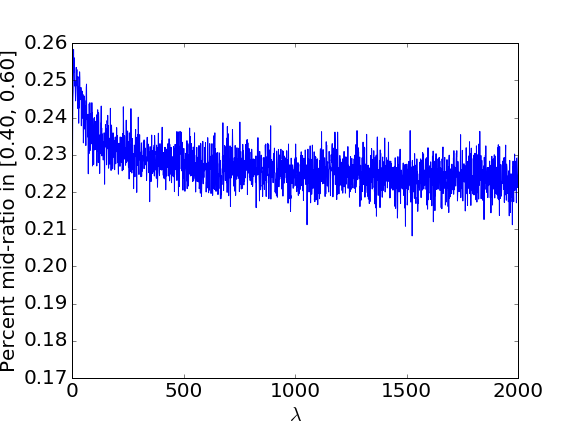
\includegraphics[width=0.5\textwidth]{midratio_sim}
    \caption{Simulated mid-ratio test}
    \label{fig:midratio}
\end{figure}
 
Carrying out this test we find that $824$ of $1362$ colony counts and $523$ of $1729$ Coulter counts produced by the RTS investigator have a mid-ratio value in the interval $\left[0.4, 0.6\right]$. If we model each triple as a Bernoulli trial with probability of success, $p = 0.26$, then the probability of observing $824$ or more successes in $1362$ colony count trials is $\expnum{1.11}{-16}$. The probability of observing $523$ or more successes in $1729$ Coulter count triplicates is $\expnum{3.26}{-5}$. These $p$-values are not reported in the paper. Both corroborate the finding that it is very unlikely that a Poisson process produced this many triplicates with mid-ratios in the interval $\left[0.4, 0.6\right]$.

While these results seem far too unlikely to have happened by chance, we are concerned by the fact that \citeauthor{Pitt:2016cu} decided to perform this test after observing ``what appeared to be an unusual frequency of triples in RTS data containing a value close to their mean.'' Other investigators besides RTS may well have trends that make their data look anomalous under these {\it post hoc} analyses. The argument would be stronger if the authors had decided what tests to perform {\it a priori}, before looking at the data and observing an ``unusual'' trend; or if they adjusted for their {\it post hoc} analysis explicitly. We believe such selection bias is not as problematic for terminal digit analysis, as it seems to be a more routine tool for investigation.

\section{Terminal Digit Analysis}

\paragraph{Assumption Check} We start by validating the assumption that the distribution of terminal digits of a Poisson variable is approximately uniformly distributed. We approximate the probability distribution of the unit digit of a Poisson variable for $\lambda$ from $50$ to $500$. Each probability distribution is compared to a uniform distribution and the total variation distance (a metric comparing the distance of distributions) is computed, and shown in \Cref{fig:term_var_dist}. The total variation distance appears relatively small, compared to $0.1$, and hence affirming the assumption.

\begin{figure}[htbp]
    \centering
    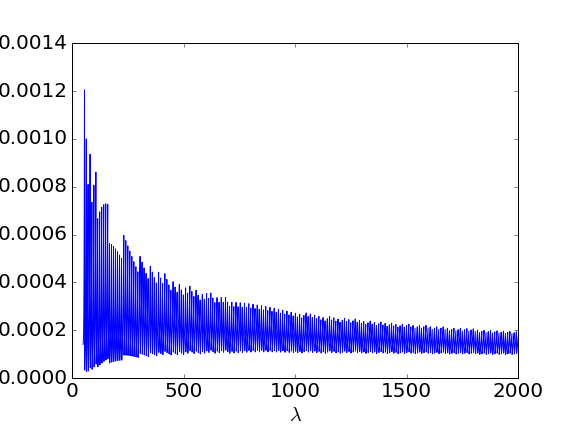
\includegraphics[width=0.5\textwidth]{term_variation_dist}
    \caption{Terminal digit variation distance from uniform distribution}
    \label{fig:term_var_dist}
\end{figure}

\paragraph{Replication} Given that the terminal digit of a Poisson distribution is approximately uniform, we replicate the chi-square goodness of fit test to assess the significance of non-uniformity in each of the data sets. Our conclusions match the findings of the paper --- we reject the null hypothesis of uniformity for the RTS data sets, and fail to reject the null for all other data sets. While our conclusions are the same, we did find some reporting issues in Table 3 of the paper. Our reproduction of Table 3 is shown in \Cref{tbl:table3}. The discrepancies between our terminal digit counts / goodness of fit calculations and the authors are shown in bold.

\begin{table}
\begin{center}
\begin{tiny}
\bgroup
\def\arraystretch{1.5} % 1 is the default
\begin{tabular}{*{14}{c}}
\hline
Data set & 0 & 1 & 2 & 3 & 4 & 5 & 6 & 7 & 8 & 9 & Total & $\chi^2$ & $p$ \\
\hline
RTS Coulter & $\bm{475}$ & $\bm{613}$ & $\bm{736}$ & $\bm{416}$ & $\bm{335}$ & $\bm{732}$ & $\bm{363}$ & $\bm{425}$ & $\bm{372}$ & $\bm{718}$ & $\bm{5185}$ & $\bm{466.9}$ & $\expnum{7.06}{-95}$ \\
Other Coulter & $261$ & $311$ & $295$ & $259$ & $318$ & $290$ & $298$ & $283$ & $331$ & $296$ & $2942$ & $16.0$ & $\expnum{6.70}{-02}$ \\
Outside Coulter 1 & $28$ & $34$ & $29$ & $\bm{25}$ & $27$ & $36$ & $44$ & $33$ & $26$ & $33$ & $\bm{315}$ & $\bm{9.476}$ & $\bm{\expnum{3.95}{-01}}$ \\
Outside Coulter 2 & $34$ & $38$ & $45$ & $35$ & $32$ & $42$ & $31$ & $35$ & $35$ & $33$ & $360$ & $4.9$ & $\expnum{8.39}{-01}$ \\
RTS Colony & $564$ & $324$ & $463$ & $313$ & $290$ & $478$ & $336$ & $408$ & $383$ & $526$ & $\bm{4085}$ & $200.7$ & $\expnum{2.33}{-38}$ \\
Other Colony & $\bm{191}$ & $\bm{181}$ & $\bm{195}$ & $\bm{179}$ & $\bm{184}$ & $\bm{175}$ & $\bm{178}$ & $\bm{185}$ & $\bm{185}$ & $\bm{181}$ & $\bm{1834}$ & $\bm{1.79}$ & $\bm{\expnum{9.94}{-01}}$ \\
Outside Colony & $21$ & $9$ & $15$ & $16$ & $19$ & $19$ & $9$ & $19$ & $11$ & $12$ & $150$ & $12.1$ & $\expnum{2.06}{-01}$\\
\hline
\end{tabular}
\egroup
\end{tiny}
\end{center}
\caption{Our replication of Table 3 from \citet{Pitt:2016cu}. Discrepancies are bolded.}
\label{tbl:table3}
\end{table}

\paragraph{Permutation Test} To bypass the assumption that the triples can be modeled as Poisson random variables, we pool all the data from all investigators and ask ``how unlikely is it that the RTS colony count terminal digits were as non-uniform as they were if they were drawn from the same distribution as all the investigators?'' The procedure for performing a permutation test is outlined as follows:

\begin{enumerate}
    \item Compute chi-squared goodness of fit test statistic for sample of interest
    \item Pool all the data
    \item Repeat the following for sufficiently many times
    \begin{enumerate}
        \item Randomly select a sample from the pooled data that is the same size as the test sample
        \item Compute the chi-squared goodness of fit test statistic for this new sample
    \end{enumerate}
    \item Find the percentage of random samples where the random sample test statistic is larger than the original test statistic
\end{enumerate}

The returned percentage approximates how likely it is that the RTS colony counts deviate more from uniformity if the counts are drawn from the same distribution as the pooled data from all the investigators. Due to limits in computing power, the number of random samples generated is limited and so is our accuracy in approximation. There were $4086$ individual RTS colony counts and $5187$ individual Coulter counts in the dataset. For $10,000$ iterations of $4086$ sample draws from the pooled investigator colony count data, the test consistently returned $0$, indicating that the RTS colony counts are consistently farther from uniform than random samples from the pooled data. The same was true for $10,000$ iterations of $5187$ sample Coulter count data.

\section{Equal Digit Analysis} 
\paragraph{Assumption Check} We question whether the assumption that the probability that the last two digits of three-plus digit Poisson variable are equal is $10\%$. To check, we performed a simulation; the results are plotted in Figure 2. When $\lambda > 500$, the probability is indeed about $10\%$, but for smaller $\lambda$, it is not.

We approximated the probability of the last two digits of a Poisson variable being equal, conditioned on the outcome bearing three digits. We plotted this in \Cref{fig:term_2dig}. While in the larger regime, where $\lambda > 500$, the probability does hover around $10\%$; the same conclusion fails to be drawn about the smaller regime.

For the equal digit analysis proposed by \citet{Pitt:2016cu} to hold, one would at least hope for this probability to be significantly different from $12.3\%$. However, when $\lambda$ gets comparable to $100$ or even smaller, this probability can rise as high as $12.5\%$. (See \Cref{fig:term_2dig}) Intuitively, if $\lambda$ is significantly smaller than $100$, then getting $100$ as an outcome is much likelier than any outcome greater than $100$, driving the probability of having the last two digits being equal much higher. Since the true $lambda$s are not known and quite a few counts are less than $100$, it is plausible that honest reporting would result in equal terminal digits more than $10\%$ of the time.

\begin{figure}[htbp]
    \centering
    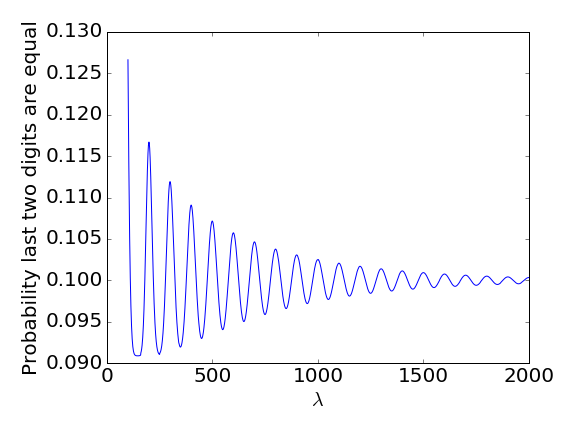
\includegraphics[width=0.5\textwidth]{term_2dig}
    \caption{Probability that two terminal digits of Poisson random variable conditional on the outcome being at least $100$ are equal}
    \label{fig:term_2dig}
\end{figure}

\section{Conclusion}

For the review process, we examine the underlying assumptions put forth by the authors. We attempt to replicate all four analyses (mid-ratio and mean counts of triplicates,  percentage of terminal digits and equal last two digits) outlined in the paper. In addition, we apply an alternative testing method that does not make assumptions on the underlying distribution of the data set, in order to check the sensitivity of the conclusions to the assumption that count triples are i.i.d.\ Poisson. 

Overall, our results agreed with those in the paper. Out of all the metrics tested, we feel that the test on percentage of terminal digits provides the strongest argument against the RTS investigator result. For the rest of the test metrics, the mid-ratio and mean counts rely on the strong assumption that each triplicate shares a common parameter $\lambda$, which we feel was inadequately justified. (The permutation test relaxes this assumption.) The expected percentage of equal last two digits of a number produced by a Poisson process, on the other hand, has a high level of inherent variability, especially if the Poisson parameter $\lambda$ that produced the data is small. Since the counts in the observed colony data are generally small ($< 200$), the percentage of equal last two digits fails to suggest any significance in the result with high level of confidence.

We feel the paper would be stronger if the authors explained in greater detail how they came to suspect RTS and how they decided to use the particular metrics they did.

Another area we did not investigate that will potentially provide additional insight is the patterns in the data of other individuals. It is possible that when examined individually, other investigators will also look anomalous for the same or other metrics. When the data are pooled together for the tests in the study, however, the individual anomalies might cancel each other out and get masked. It will therefore be useful for future studies / reviews to conduct further investigation in this area.

\section*{Reproducibility}
The source code for our analysis can be found below:\\ \url{https://github.com/mads14/Science_Open_Referee_Report}

The original full datasets for the study can be found below:\\ \url{https://osf.io/mdyw2/files/}.

\section*{Acknowledgement and Declaration}
We would like to thank the authors for making their data available and for publishing in an open journal.

This review was vetted by Philip B Stark. However, the work was conducted entirely by the authors, and the opinions expressed in this review are those of the authors.

\bibliographystyle{plainnat}
\bibliography{bib}

\end{document}